\documentclass[12pt,a4paper]{article}
\usepackage[utf8]{inputenc}
\usepackage[spanish]{babel}
\usepackage[margin=0.5in, top=0.5in, bottom=0.5in]{geometry}
\usepackage{amsmath}
\usepackage{amsfonts}
\usepackage{amssymb}
\usepackage{hyperref}
\usepackage{graphicx}
\usepackage[shortlabels]{enumitem}
\newcommand{\p}{\phantom{......}}

\title{Bases de datos 2023-1\\
Práctica 1: Bitácora}
\begin{document}
\maketitle

\textbf{Reporte de instalación:}\\
\begin{enumerate}
	\item \textit{Sistema operativo y versión:} MacOS Monterrey v12.5\\


	\item \textit{Versión de la instalación:} psql (PostgreSQL) 14.5\\

	\item \textit{Tiempo requerido:} 5min\\

	\item \textit{Paso a Paso:}\\
		Primero busque y descargue el instalador para MacOs 
		
		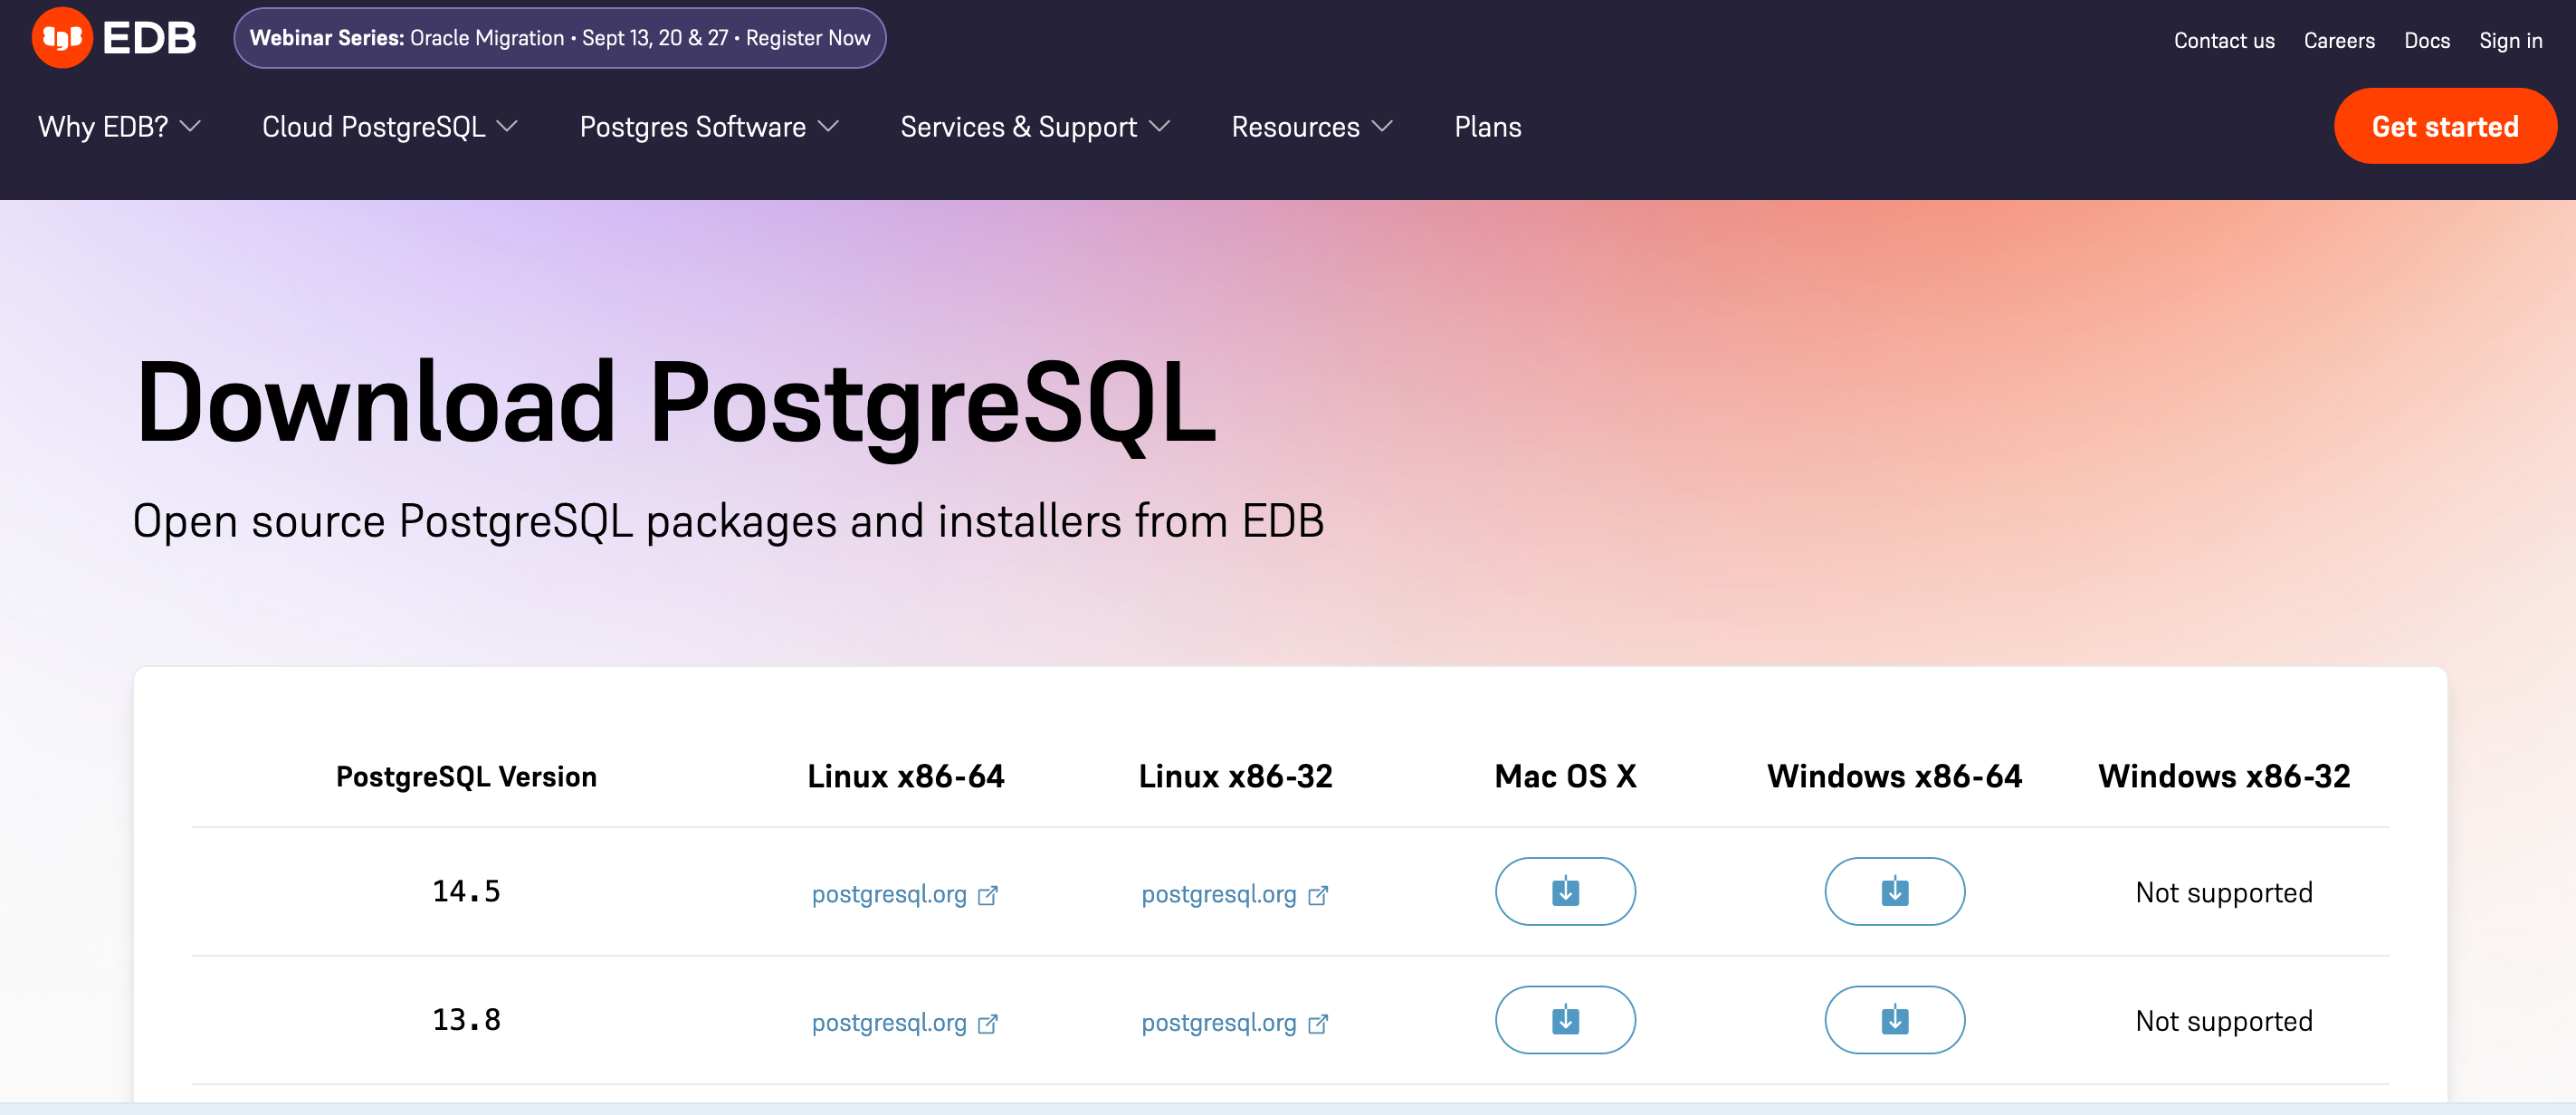
\includegraphics[scale=0.2]{assets/step01.png}

		Luego simplemente seguí todos los pasos del instalador:\\
		
		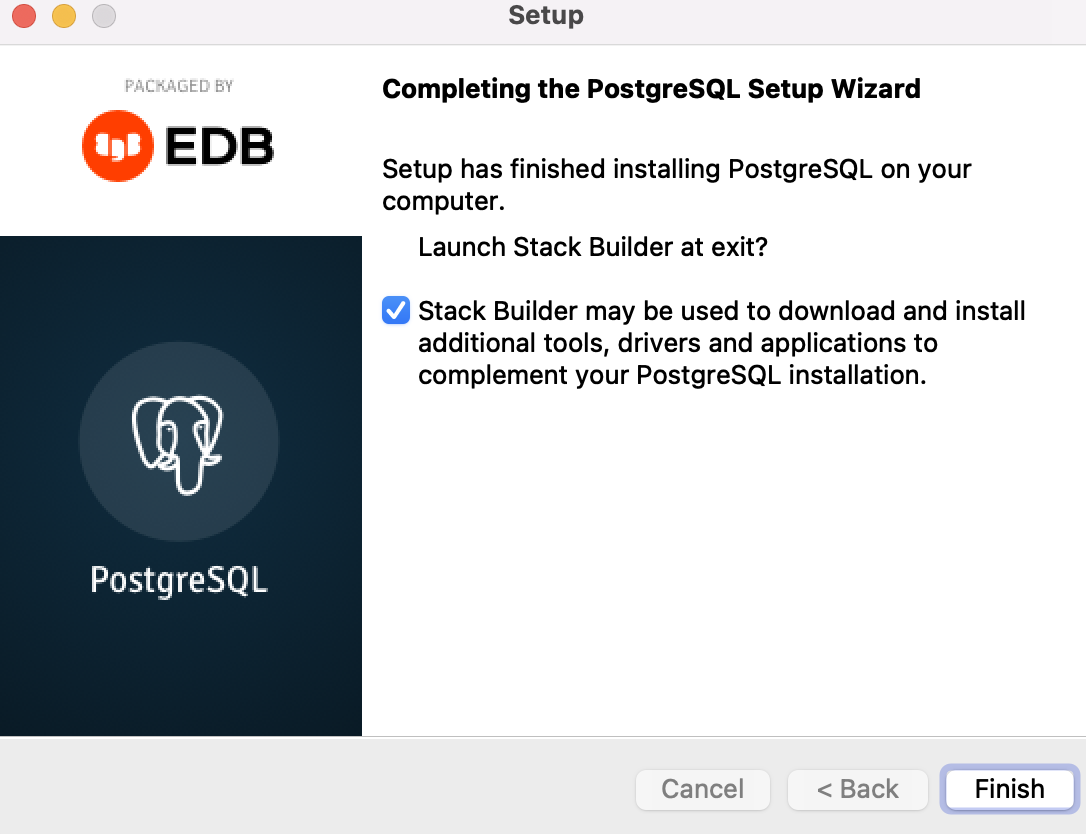
\includegraphics[scale=0.3]{assets/step02.png}

	    Despues abri pgAdmin 4 para verificar que todo funcionara
	
		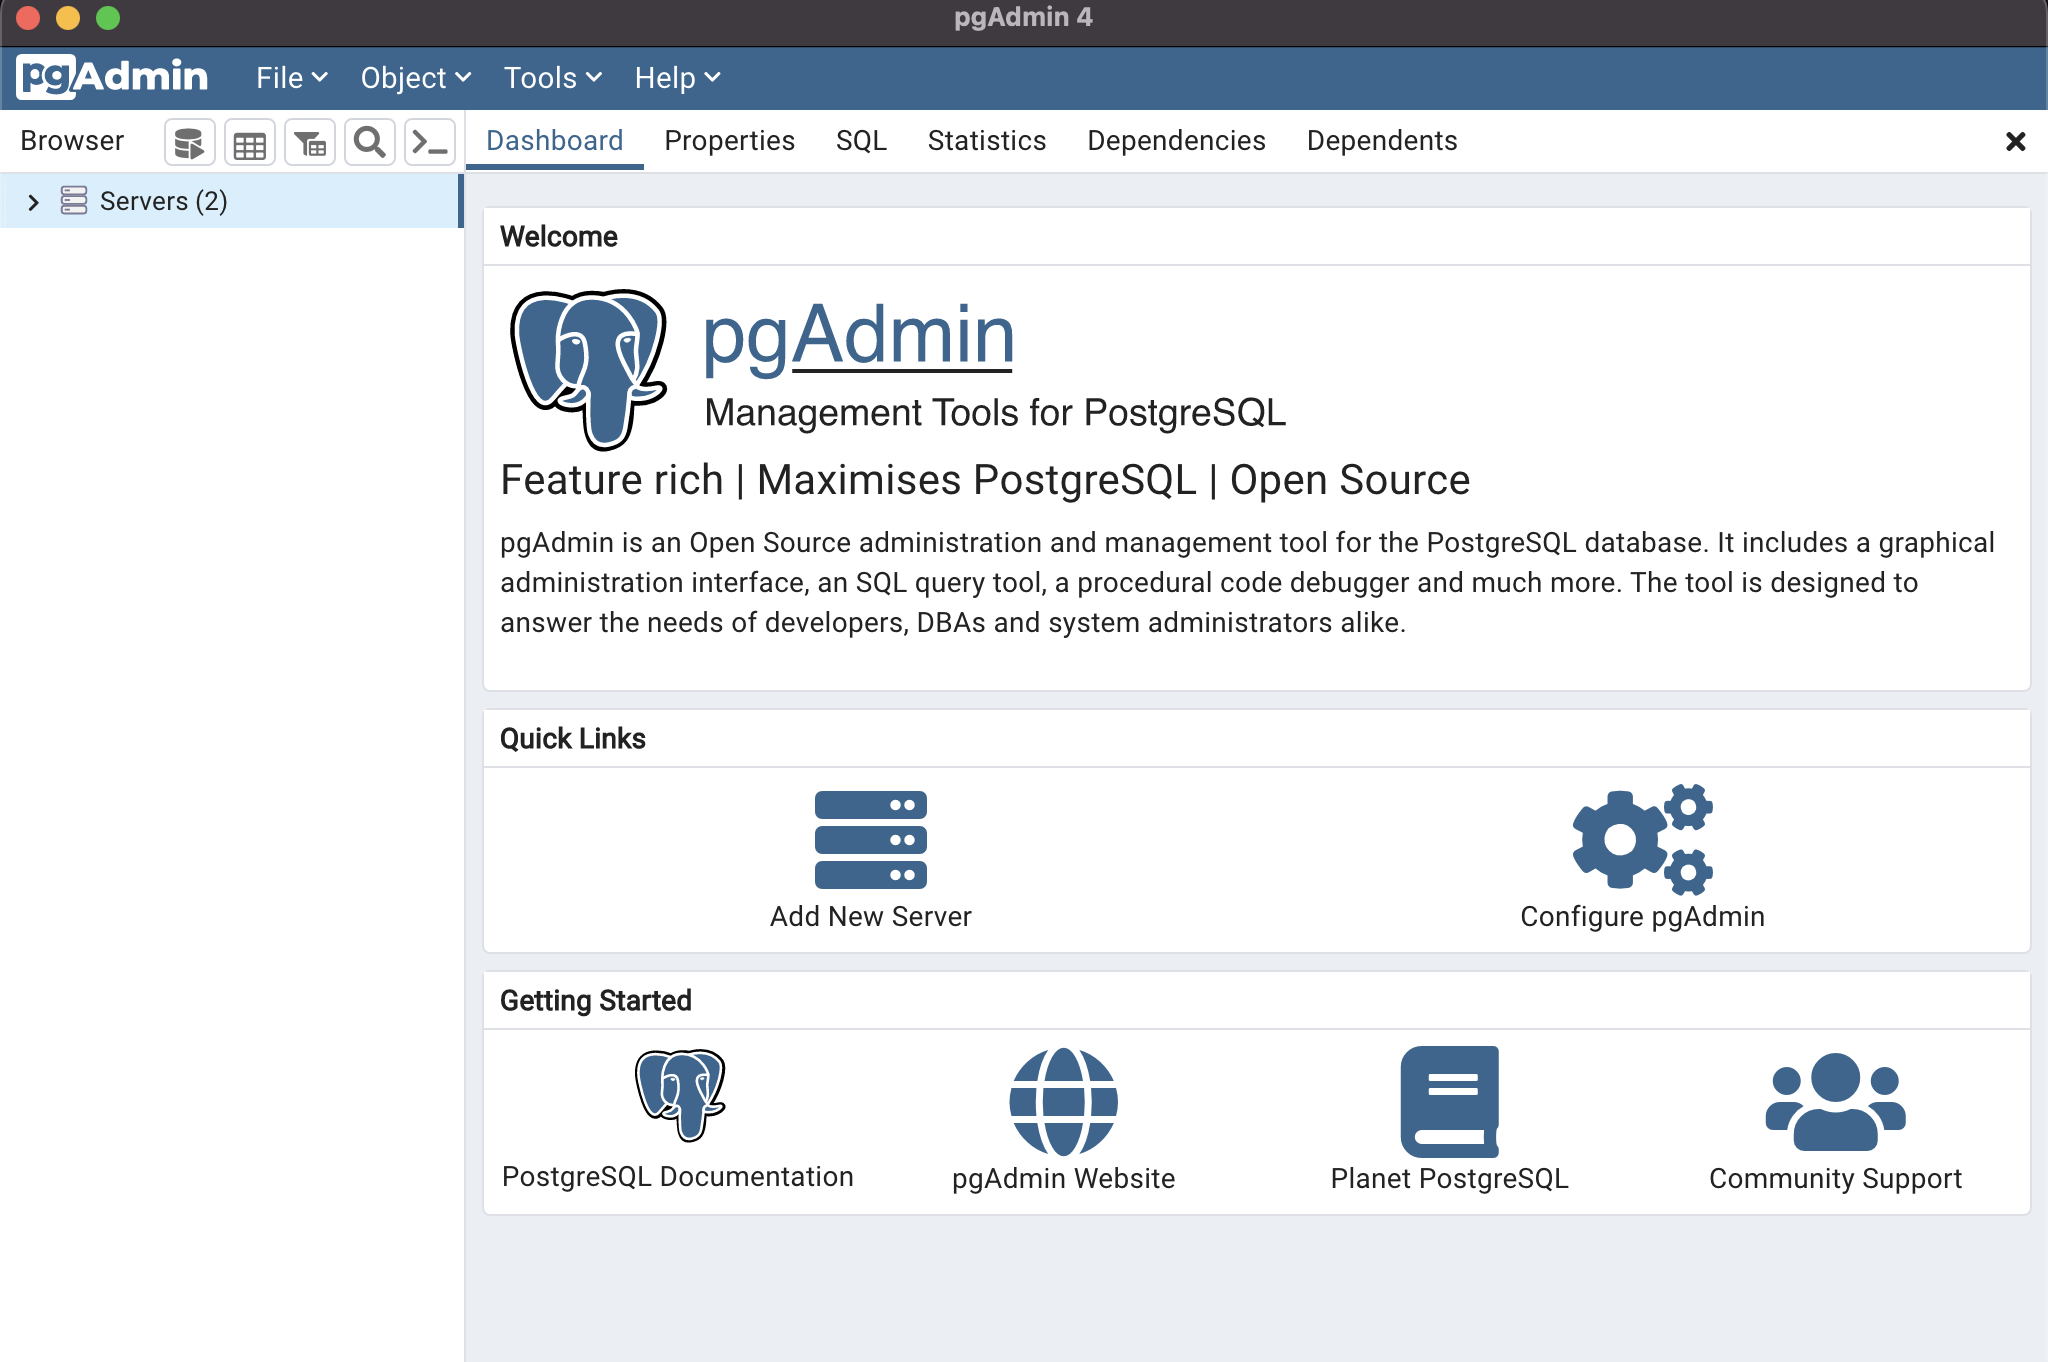
\includegraphics[scale=0.3]{assets/step03.png}

	

	\item \textit{Comentarios y problemas:}\\
		No teuve ninguna compliacion, afortunadamente ya no hay problemas de compatibilidad con los chips M1 de Apple.
\end{enumerate}

\end{document}